In contrast to muon CLFV searches, in which a single dedicated experiment is required for a given decay,  $\tau$~lepton CLFV searches are conducted using the large data sets collected in comprehensive $e^+e^-$ or hadron collider experiments. The relative theoretical parameter reach of $\mu$ and $\tau$ decay experiments is model-dependent, and thus comparisons of limits or observations in the two cases can serve to distinguish between models.
Tests with taus can be more powerful on an event-by-event basis than those using muons, since the large $\tau$ mass greatly decreases 
Glashow-Iliopoulos-Maiani (GIM) suppression, correspondingly increasing new physics partial widths (typically by a factor of $\geq 500$ in $\cal{B}(\tau \rightarrow \mu \gamma)$ or $e \gamma$ {\it vs.} $\cal{B}(\mu \rightarrow e \gamma$)).  The difficulty is that one can typically produce $\sim 10^{11}$ muons per second, while the samples from \babar\ and Belle collected over the past decade together total $\sim 10^{10}$ events.  

The new generation of super $B$ or $\tau$/$c$ factories, \cite{ref:superkekb} promise to extend the
experimental reach in $\tau$ decays to levels that sensitively
probe new physics in the lepton sector. Since CLFV is severely suppressed in the Standard Model, CLFV $\tau$ decays
are especially clean probes for New Physics
effects.  The
super flavor factories can access $\tau$ CLFV decay rates two orders of magnitude smaller than current limits for the cleanest channels
({\it e.g.}, $\tau\to 3\ell$), and at least one order of magnitude smaller for other
modes that have irreducible backgrounds, such as $\tau\to \ell\gamma$. Super flavor factories thus have a sensitivity for CLFV decays that directly confronts many NP models. 

Polarized beams at an $e^+e^-$ collider can provide further
experimental advantages.   Belle II at \hbox{SuperKEKB} will not have a polarized beam, but both the proposed BINP and Tor Vergata $\tau$/$c$ factories will have polarized electron beams.  Polarization of the taus thus produced provides several advantages. It allows reduction of backgrounds in certain
CLFV decay modes, as well as providing sensitive new
observables that increase precision in other important measurements, including
searches for $C\!P$ violation in $\tau$ production and decay, the measurement
of $g-2$ of the $\tau$, and the search for a $\tau$ EDM.  Preliminary studies indicate that polarization improves the sensitivity on these quantities by a factor of two to three. Should the CLFV decay $\tau \rightarrow 3\ell$ be found, a study of the Dalitz plot of the polarized $\tau$ decay can determine the Lorentz structure of the CLFV coupling.

The provision of polarization requires a polarized electron gun, 
a lattice that supports transverse
polarization at the desired CM energy, a means of interchanging transverse polarization in the
ring and longitudinal polarization at the interaction point and a means of monitoring
the polarization, typically a Compton polarimeter to monitor the
backscattering of circularly polarized laser light. Achieving useful longitudinal polarization at the interaction point requires sufficiently long depolarization time of the machine lattice, which is highly dependent on the details of the lattice and the beam energy.

Provision of a
polarized positron beam is difficult and expensive; it is generally
also regarded as unnecessary, as most of the
advantages of polarization for the measurements cited above can be
accomplished with a single polarized beam.

\begin{figure}[htb]

\begin{center}
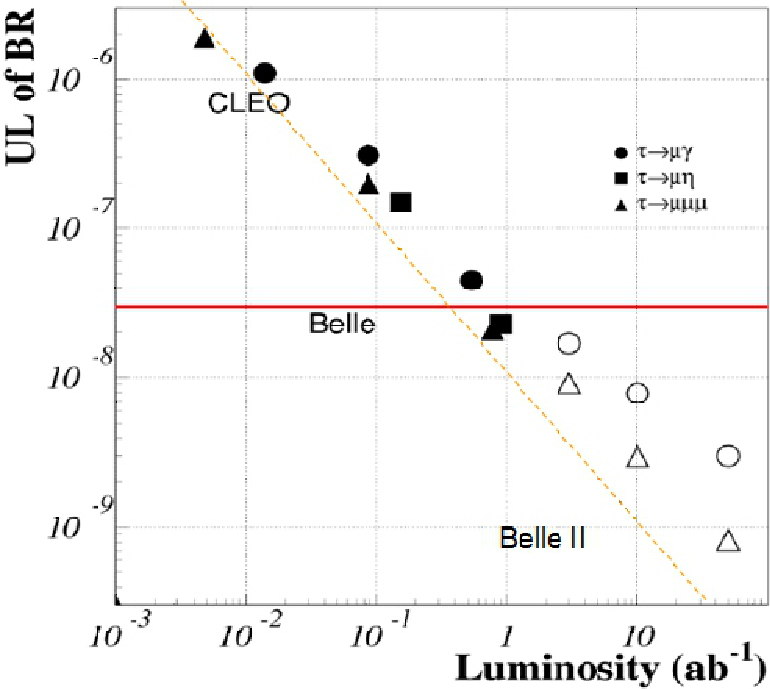
\includegraphics[width=8cm]{ChargedLeptons/Figures/Belle-tau.pdf}
\smallskip
\caption{\label{CL:Belle}Extrapolationn of the 90\% upper limit sensitivity of Belle-II (open symbols) from existing limits (filled symbols). For $\tau\rightarrow \mu\gamma$, which has irreducible backgrounds, the limit scales as $1/{\sqrt{\!\int{\!\cal{L}}dt}}$. For $\tau\rightarrow \mu\mu\mu$, which is essentially background-free, the limit scales as $1/{\int{\!\cal{L}}dt}$.}
\end{center}
\end{figure}

The sensitivity of $\tau$ CLFV searches at SuperKEKB has been estimated by extrapolating from current CLEO, Belle and \babar\  
limits (see Figure~\ref{CL:Belle} The optimization of search sensitivities depends on the size
of the sample as well as on the sources of background. For SuperKEKB, the
extrapolation for the (largely background-free) $\tau\to\ell\ell\ell$
modes assumes $1/{\mathcal L}$ scaling up to 5 ab$^{-1}$; that for $\tau\to\ell\gamma$
modes scales as $1/{\sqrt{\mathcal L}}$. 
The expected sensitivities for several modes are shown for the Belle II experiment in Table~\ref{tab:LFVExptSensitivities-BelleII}~\cite{Abe:2010sj}.  

\begin{table}[!b]
  \caption{
    \label{tab:LFVExptSensitivities-BelleII}
    Expected $90\%$ CL upper limits
    on $\tau\to\mu\gamma$, $\tau\to \mu\mu\mu$, and $\tau\to \mu\eta$
    with $5 \ {\rm ab}^{-1}$ and  $50 \ {\rm ab}^{-1}$ data sets from Belle II and  Super KEKB.
  }
  \begin{center}
    \begin{tabular}{lll}
      \hline \hline
Process & $5\ {\rm ab}^{-1}$ & $50\ {\rm ab}^{-1}$  \\
      \hline
      $\BR(\tau \to \mu\,\gamma) \rule{0pt}{2.6ex}$ &  $10 \times 10^{-9}$ &  $3 \times 10^{-9}$  \\
      $\BR(\tau \to \mu\, \mu\, \mu)$ &  $3 \times 10^{-9}$ & $1 \times 10^{-9}$  \\
      $\BR(\tau \to \mu \eta)$             &  $5 \times 10^{-9}$ & $2\times 10^{-9}$    \\
 \hline\hline
    \end{tabular}
  \end{center}
\end{table}


These CLFV sensitivities directly confront a large variety of new
physics models. Of particular interest is the correlation between
$\tau$ CLFV branching ratios such as $\tau\to \mu\gamma$ and $\tau\to e
\gamma$, as well as the correlation with $\mu\to e \gamma$ and the
$\mu\to e$ conversion rate, all of which are diagnostic of particular
models.  A polarized electron beam potentially allows the possibility of determining the helicity structure of CLFV couplings from Dalitz plot analyses of, for example, $\tau \to 3\ell$ decays.

The experimental situation at a $\tau/c$ factory is somewhat different. The luminosity of the proposed projects is $10^{35}$cm$^{-2}$s$^{-1}$, a factor of eight below the eventual SuperKEKB luminosity. The $\tau$ production cross section is, however, larger: $\sigma_{\tau\bar{\tau}}(3.77\  \gev)/\sigma_{\tau\bar{\tau}}(10.58\  \gev)=3$, and both have a polarized electron beam. In addition, while a Super $B$ factory is likely to spend the bulk of its running time at the $\Upsilon(4S)$, a $\tau/c$ factory will take data more evenly throught the accessible energy range.  A study for the BINP machine, with 1.5 ab$^{-1}$ at 3.686 GeV,
3.5 ab$^{-1}$ at 3.770 GeV, and 2.0 ab$^{-1}$ at 4.170 GeV, 
corresponding to  $2.5\times 10^{10}$ produced $\tau$ pairs, quotes a 90\% confidence level limit on $\cal{B}(\tau\rightarrow\mu\gamma)$= $(3.3\times 10^{-10})$, provided the detector has $\mu/\pi$ rejection of a factor of 30. This is nearly an order of magnitude improvement over the SuperKEKB expectation at 50 ab$^{-1}$.


The experimental discrepancy with the Standard Model prediction for
the muon anomalous magnetic moment heightens interest in the
possibility of measuring $g-2$ of the $\tau$ lepton using angular
distributions in $\tau$-pair production. This can be done at a super flavor factory, with or without electron polarization.  With polarized taus one can access new observables that are estimated by
Bernab\'eu {\it et al.}\cite{ref:b1} to increase the sensitivity to
$g-2$ by a factor of three, to $\sim2\times 10^{-6}$ with 80\%
electron polarization, which could allow a measurement of the Standard
Model moment to a precision of several percent with a data sample of
75 ab$^{-1}$.

Observation of a $\tau$ EDM would be evidence of $T$ violation.  $T$-odd observables can be isolated by the study of $\tau$ angular
distributions using unpolarized beams. Having a polarized electron
beam allows these investigations to be done using the decay products
of individual polarized taus.  The upper-limit sensitivity for the real part of the
$\tau$ EDM has been estimated to be to be $|\Re{d_\gamma}|\simeq 3\times 10^{-19} \ e \cdot {\rm cm}$
with 50 ab$^{-1 }$ at Belle II and $|\Re{d_\gamma}|\simeq 7\times 10^{-20} \ e \cdot {\rm cm}$
with 75 ab$^{-1 }$ at Super$B$\cite{ref:b2}.

A $C\!P$-violating asymmetry in $\tau$ decay would be manifest evidence
for physics beyond the Standard Model. \babar\ has recently published
a 3$\sigma$ asymmetry in $\tau\to\pi K_S^0(\ge 0\pi^0)$
decay\cite{ref:taucp}. The super flavor factories have the sensitivity to
definitely confirm or refute this measurement, and, further, provide
access to new $C\!P$-odd observables that increase the sensitivity in the
search for a $C\!P$ asymmetry to the level of $\sim 10^{-3}$.
